\chapter{Arhitectura Software}
\thispagestyle{pagestyle}

Arhitectura software generală a sistemului este alcătuită la rândul ei din trei arhitecturi software separate: arhitectura software pentru placa de dezvoltare Arduino Mega, arhitectura software pentru aplicația mobilă și arhitectura software pentru platforma web/mobile Blynk. În acest capitol ne vom axa doar pe arhitectura generală.

În Figura \ref{fig:arhitectura_soft_general} este prezentată schema bloc a sistemului. Practic, se poate observa funcționarea sistemului într-un ciclu de execuție. Flow-ul de execuție al unui ciclu este următorul: se alimentează sistemul, se inițializază placa, modulele și senzorii, se stabilesc conexiunile cu NodeMCU și modulul de Bluetooth; dacă tot acest setup este efectuat cu succes urmează să introducem un număr la tastatură. Acest număr reprezintă temperatura de prag pe care o dorim în casă. Acest proces de introducere al numărului se termină în momentul în care este apăsată tasta "\#". După introducere, microcontrolerul strânge datele de la senzori, afișează aceste date pe LCD, după care comandă actuatorii (leduri, buzzer, servomotor).

Următorul pas este încercarea de a trimite date prin modulul de Bluetooth către aplicația mobilă de Android. Dacă transmisia a fost realizată cu succes, aplicația va afișa pe ecran datele primite și va aștepta următoarea transmisie lăsând microcontrolerul să execute instrucțiunile rămase. Dacă transmisia eșuează, microcontrolerul ignoră acest fapt continuând setul de instrucțiuni, astfel sistemul nu rămâne blocat.

Apoi, microcontrolerul va încerca să trimită datele către NodeMCU. Dacă comunicarea este realizată cu succes, NodeMCU va trimite datele mai departe către Serverul Blynk, iar acesta le va afișa în interfața platformei. Pe urmă, NodeMCU așteaptă date noi permițând microcontrolerului să execute programul rămas. Dacă comunicarea nu se poate realiza între cele două, microcontrolerul ignoră acest pas și continuă.

Ultima etapă este cea de verificare: dacă palca de dezvoltare este alimentată va continua repetarea acestui ciclu. Astfel, atât timp cât Arduino Mega este alimentată sistemul va executa ciclic aceste etape până la un semnal de reset sau oprirea alimentării.

\begin{figure}[H]
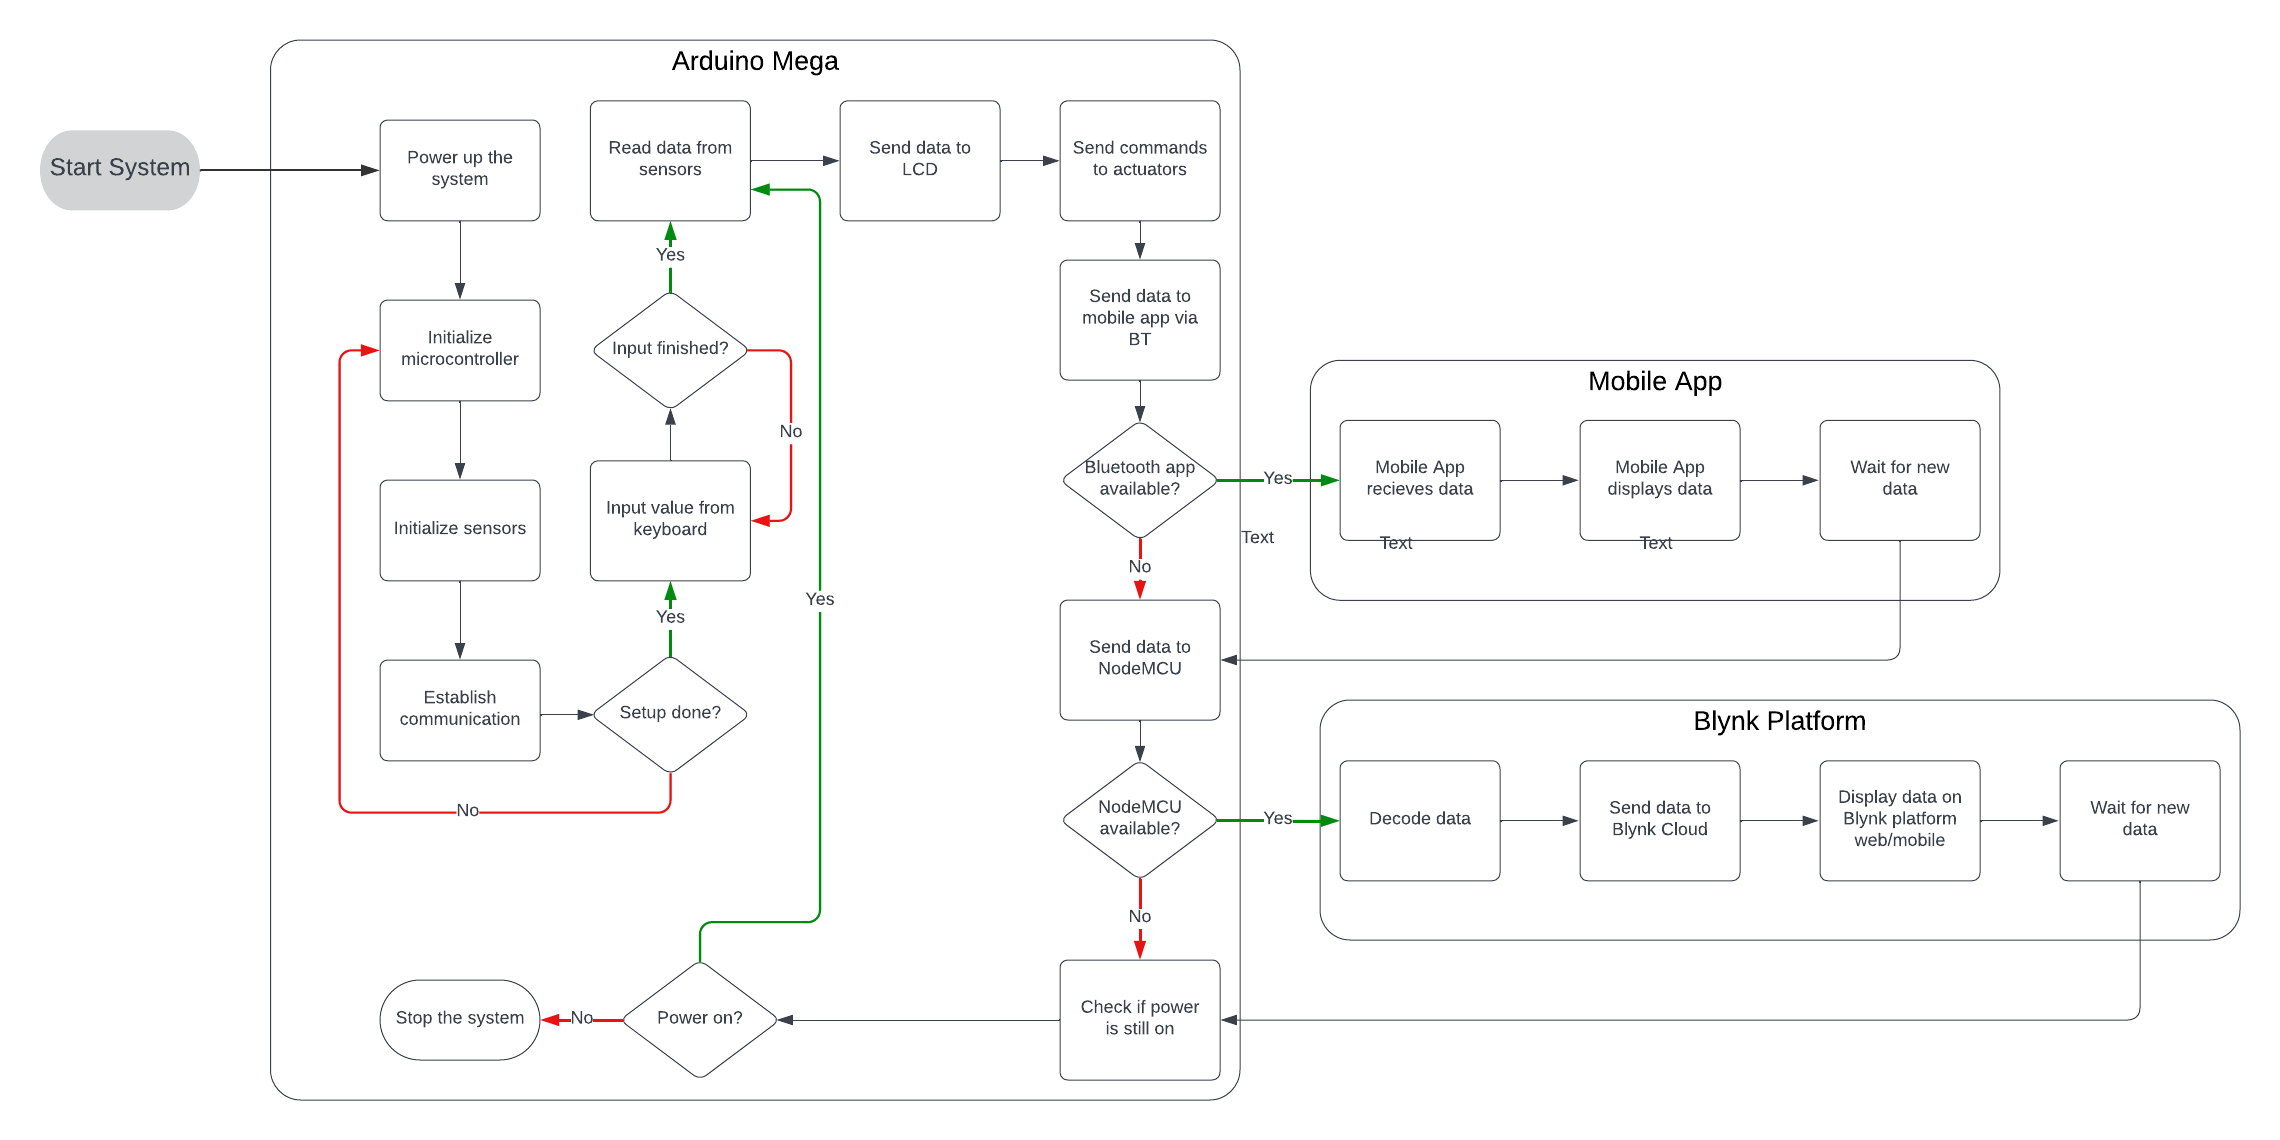
\includegraphics[width=1\textwidth, height=0.6\textwidth]{bachelors_ro/images/arhitectura_soft_general.png}
\caption{Schema software bloc a sistemului}
\label{fig:arhitectura_soft_general}
\end{figure}
